\documentclass{tufte-handout}

\title{Human-level control through \\ deep reinforcement learning}

\author[Marius Stanescu]{Marius Stanescu}
%\date{28 March 2010} % without \date command, current date is supplied
%\geometry{showframe} % display margins for debugging page layout

\usepackage{graphicx} % allow embedded images
  \setkeys{Gin}{width=\linewidth,totalheight=\textheight,keepaspectratio}
  \graphicspath{{graphics/}} % set of paths to search for images
\usepackage{amsmath}  % extended mathematics
\usepackage{booktabs} % book-quality tables
\usepackage{units}    % non-stacked fractions and better unit spacing
\usepackage{lipsum}
\usepackage{multicol} % multiple column layout facilities
\usepackage{fancyvrb} % extended verbatim environments
  \fvset{fontsize=\normalsize}% default font size for fancy-verbatim environments

% Standardize command font styles and environments
% \newcommand{\doccmd}[1]{\texttt{\textbackslash#1}}% command name -- adds backslash automatically
% \newcommand{\docopt}[1]{\ensuremath{\langle}\textrm{\textit{#1}}\ensuremath{\rangle}}% optional command argument
% \newcommand{\docarg}[1]{\textrm{\textit{#1}}}% (required) command argument
% \newcommand{\docenv}[1]{\textsf{#1}}% environment name
% \newcommand{\docpkg}[1]{\texttt{#1}}% package name
% \newcommand{\doccls}[1]{\texttt{#1}}% document class name
% \newcommand{\docclsopt}[1]{\texttt{#1}}% document class option name
% \newenvironment{docspec}{\begin{quote}\noindent}{\end{quote}}% command specification environment


%------------------ STUFF YOU CAN USE IN TUFTE --------------------------------
% \section{}
% \subsection{}
% \newthought{}
% \footnote{}
% \marginnote[Vertical_offset]{text}
% \sidenote[number][Vertical_offset]{text}
% \cite[V_offset]{bla,bla}
% \begin{fullwidth}
% figure, table
%  with * -> full page
% marginfigure, margintable
% \begin{marginfigure}[V_offset]
%   \includegraphics[width=\linewidth]{name}
%   \caption{}
%   \label{fig:}
% \end{marginfigure}
% \smallcaps{}
% \textsc{}
% \url{https://github.com/Tufte-LaTeX/tufte-latex}
% -----------------------------------------------------------------------------


\begin{document}

\maketitle% this prints the handout title, author, and date
%------------------------------------------------------------------------------
\begin{abstract}
\noindent
In this document  I will give a brief outline of the 2015 Nature paper mentioned in the title  \cite{Mnih2015-fy}. These notes are taken for the Bucharest Computer Vision meet-up organized on the 16th of March, 2017. Since this is the first reinforcement learning paper discussed with the group, I focus more on the basic RL required to understand the paper and the intuition of why the DQN algorithm works. More implementation details or technical elements can be found in the paper or explored in a later meeting.

\end{abstract}
%------------------------------------------------------------------------------
Mnih et al. first introduced the Deep Q-Network (DQN) algorithm in 2013 \cite[-0.5cm]{Mnih2013-ts}, and the result received a lot of attention as it came when the deep learning craze was starting to take off\marginnote[0.1cm]{There were some breakthrough publications in computer vision and speech recognition such as AlexNet (2012), ImageNet competition etc.}. Their work is based on Q-value iteration and it was applied to ATARI games helping establish ALE(Arcade Learning Environment) as an RL benchmark~\cite[0.2cm]{Bellemare2013-wj}. A single architecture (same algorithm, network architecture and hyperparameters) can be used to play 47 ATARI games, more than half at or above human level. The screen is taken as input (pixel level) and Q-values are returned as output (think goodness of all actions). It outperforms classic RL methods\sidenote[][1cm]{Note that these are quite weak baselines, if we look at what we have now after tuning/improving for a couple years on this dataset} that use hand-crafted features without any game-specific knowledge, just by processing the screen pixels.

This document continues with an introduction to RL, building up from basics up to Q-value iteration and some of its modifications required to understand DQN. This is followed by a short explanation of DQN and what improvements in makes, a brief overview of the paper's results and a few conclusions and tips. But first, let's talk about the core concepts of reinforcement learning.

%==============================================================================
\section{What is Reinforcement Learning (RL)?}
%==============================================================================
\begin{marginfigure}[2cm]
  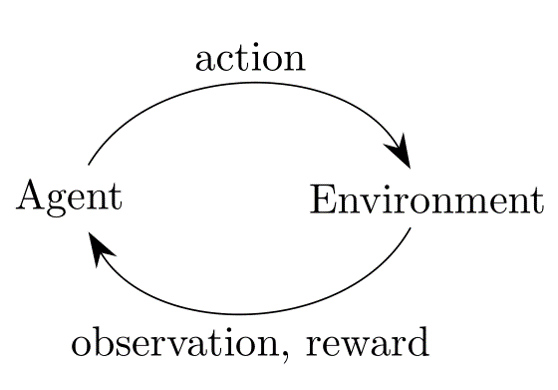
\includegraphics[width=\linewidth]{RL}
  \caption{RL - an iterative trial and error process.}
\end{marginfigure}
Reinforcement Learning is an exciting area of machine learning. Informally, it's about learning an efficient strategy (sequences of actions) in a given environment you may or may not know the physics of\marginnote{Compared to supervised learning we usually don't have full access to function to be optimized and need to query it through interaction}. Rewards are assigned for a given behavior and  over time, the agents learns to reproduce that behavior in order to receive more rewards. 

%==============================================================================
\section{MDPs and terminology}
%==============================================================================
Formally, an environment is defined as a Markov Decision Process (MDP) or Partially Observed MDP (POMDP):
\begin{itemize}
  \item $\mathbf{S}$ - set of states of the environment
  \item $\mathbf{A}$ - set of actions, which the agent selects from at each time step
  \item $\mathbf{P(r,s'|s,a)}$ - a transition probability distribution of receiving a reward $r$ and transition to $s'$ \marginnote[-0.5cm]{In a deterministic environment (chess) this will look like a delta function (1 for $s'$ and 0 everywhere else). Also, $P$ can also be provided as $P(s'|s,a)$ and one of $R(s), R(s,a) \text{ or } R(s,a,s')$.}
  \item $\gamma$ - a discount factor $\gamma \in (0,1)$, indicating preference for present rewards compared to future rewards
\end{itemize}

Other terminology:
\begin{itemize}
  \item[\textbf{Episode}] - a complete play from one of the initial states to a final state $(s_0,a_0,r_0), (s_1,a_1,r_2), \ldots, (s_n)$.

  \item[\textbf{Cumulative (discounted) reward}] - also called return, it is the (discounted) sum of reward accumulated throughout an episode $R = r_0 +  r_1 + \ldots + r_{T-1} + V(s_T) $ or  $R =  r_0 + \gamma r_1 + \gamma^2 r_2 + \ldots $
    \marginnote{The goal is to find the optimal policy $\pi^*$ that maximizes the expected return: $\max_{\pi} E [ r_0 + \gamma r_1 + \gamma^2 r_2 + \ldots ]$. This is usually intractable, so we need to train an agent such that his policy converges to the theoretical optimal policy.}
    \vspace{-10pt}

  \item[\textbf{Policy} $\pi$] - the agent's strategy to choose an action at each state, can be stochastic $\pi(a|s)$ or deterministic $\pi(s)=a$.

  \item[\textbf{Sate value function} $V^\pi(s)$] - the expected cumulative reward from a state $s$ following that policy
    \marginnote{Say we have $V^*$ the value function of the optimal policy $\pi^*$. If we want to retrieve $\pi^*$ we can do so greedily by choosing $a = arg \max_a[E_\pi(r_0 + \gamma V(s_{1}))]$. However, in the model-free setting we don't know $s_{1}$, so that's why we need Q functions. We can now retrieve $\pi^*$ by $a = arg \max_a [Q^{\pi^*}(s_0,a)]$. No more uncomputable expectations, cool! We moved the expectation inside Q, which we now hope is smooth enough to be reasonably approximated with NNs.} 
    \begin{align*}
    V^\pi(s_0) &= E_\pi [ r_0 + \gamma r_1 + \gamma^2 r_2 + \ldots ] \\
    &= E_\pi [ r_0 + \gamma V(s_{1}) ] \\
    &= \max_a Q^\pi(s_0,a)
    \end{align*}

  \item[State-action value function] - also called \textbf{Q function} 
    \begin{align*}
    Q^\pi(s_0,a_0) &= E_{s_1\sim P(s_1|s_0,a_0)} [ r_0 + \gamma r_{1} + \gamma^2 r_{2} + \ldots] \\
    &= E_{s_1\sim P(s_1|s_0,a_0)} [ r_0 + \gamma V^\pi(s_{1})] \\
    &= E_{s_1\sim P(s_1|s_0,a_0)} [ r_0 + \gamma E_{a_{1}\sim\pi} [Q^\pi(s_{1},a_{1})]] 
    \end{align*}
\end{itemize}

%==============================================================================
\section{Bellman equation and backups}
%==============================================================================
The equation 
\vspace{-5pt}
  \begin{align*}
  Q^\pi(s_0,a_0) = E_{s_1\sim P(s_1|s_0,a_0)} [ r_0 + \gamma E_{a_{1}\sim\pi} [Q^\pi(s_{1},a_{1})]]
  \end{align*}
is called the Bellman equation. For an optimal policy $\pi^*$ we can define the optimal $Q^* = Q^{\pi^*}$ which satisfies $Q^*(s,a) = \max_\pi Q^\pi(s,a)$. As hinted to in the sidenotes, $\pi^*(s)= arg \max_a Q^*(s,a) $. We can re-write the Bellman equation for $Q^*$ as:
\vspace{-5pt} 
  \begin{align*}
Q^*(s_0,a_0) = E_{s_1\sim P(s_1|s_0,a_0)} [ r_0 + \gamma \max_{a_{1}} Q^*(s_{1},a_{1})]
  \end{align*} 
The optimal strategy is to select $a_1$ that maximizes the expected value. Next, the Bellman backup operator $\mathcal{T}$ applied to a function $Q$ is 
\vspace{-15pt}
  \begin{align*}
  [\mathcal{T} Q](s_0,a_0) = E_{s_1\sim P(s_1|s_0,a_0)} [ r_0 + \gamma \max_{a_{1}} Q(s_{1},a_{1})].
  \end{align*} 
It can be proved that $Q^*$ is a fixed point of this operator,  meaning that $\mathcal{T} Q^* = Q^*$. Moreover, if we apply this operator to any initial $Q$, the series converges to $Q^* \,$: $\, Q,\,\mathcal{T} Q,\,\mathcal{T}^2 Q, \ldots \rightarrow Q^*$. 

%==============================================================================
\section{Q-Value iteration}
%==============================================================================
We now have all the ingredients for the basic version of Q-value iteration: start with a random $Q$ and iteratively apply $\mathcal{T}$ until convergence. This works because we can greedily compute $\max_a Q(s,a)$ inside $\mathcal{T}$, even without knowing the transition probabilities (model-free RL).
\begin{marginfigure}[-1.5cm]
  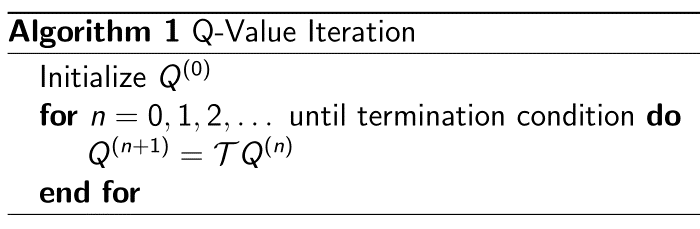
\includegraphics[width=\linewidth]{Qv}
  \caption{Q-Value iteration}
\end{marginfigure}

We can compute an unbiased estimator of the RHS in the Bellman equation using a single sample -- a single transition $(s,a,r,s')$ --, and it does not matter what policy was used to select actions (off-policy): 
  \begin{align*}
    [\widehat{\mathcal{T} Q}](s_0,a_0) =  r_0 + \gamma \max_{a_{1}} Q(s_{1},a_{1})
  \end{align*}
 Backups still converge to $Q^*$ even with this noise! \cite{Jaakkola1994-nc}

Then, in the first version of Q-Value we replace $Q^{(n+1)} = \mathcal{T} Q^{(n)}$ by 
  \begin{align*}
  Q^{(n+1)}(s,a) &= mean \{\widehat{\mathcal{T} Q_t}, \forall t \text{ such that } (s_t,a_t)=(s,a)\}  \\
  & \text{ and } \widehat{\mathcal{T} Q_t} = r_t + \gamma \max_{a_{t+1}} Q^{(n)}(s_{t+1},a_{t+1}).
  \end{align*}
The mean is computed after interacting with the environment for a fixed number of timesteps $K$, and for all $(s,a)$ pairs.  This is known as sampling-based Q-value iteration.

Next, we want to parameterize $Q$ with a network $Q_\theta$, instead of using a tabular form. For it to work, we need to rephrase this as an optimization problem \footnote{Recall that we can express \\  $mean\{\hat{x_i}\} = arg \min_x \sum_i \| x_i-x\|^2$}:
\begin{marginfigure}[0cm]
  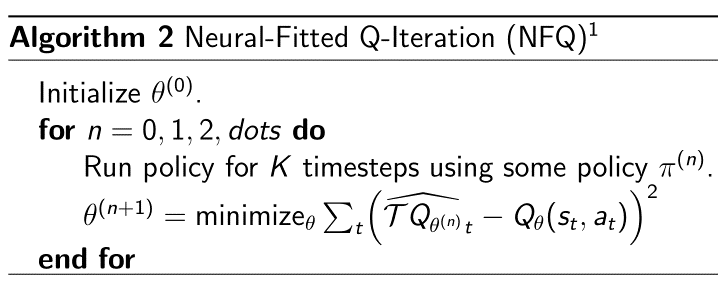
\includegraphics[width=\linewidth]{nfq}
  \caption{Neural-Fitted Q-Iteration}
\end{marginfigure}
\vspace{-20pt}
  \begin{align*}
    Q^{(n+1)}(s,a) = arg \min_{Q} \sum_{t=1}^{K} \| \widehat{\mathcal{T} Q_t} - Q(s_t,a_t) \|^2
  \end{align*}
The resulting batch algorithm is called Neural-Fitted Q-Iteration \cite{Riedmiller2005-lk}.

Finally, we can adapt this batch method into an online/incremental algorithm in which we can simply plug SGD, for example. Instead of the full backups $Q = \widehat{\mathcal{T} Q_t}$ we were doing before, we can do a partial backup:
\vspace{-23pt}
\begin{align*}
Q &= \epsilon \widehat{\mathcal{T} Q_t} + (1-\epsilon)Q \\
  &= Q - \epsilon (Q - \widehat{\mathcal{T} Q_t} ) \\
  &= Q - \epsilon \nabla_Q \| Q - \widehat{\mathcal{T} Q_t} \|^2 / 2
\end{align*} which is equivalent to a gradient step on the squared error. 
\begin{marginfigure}[-3cm]
  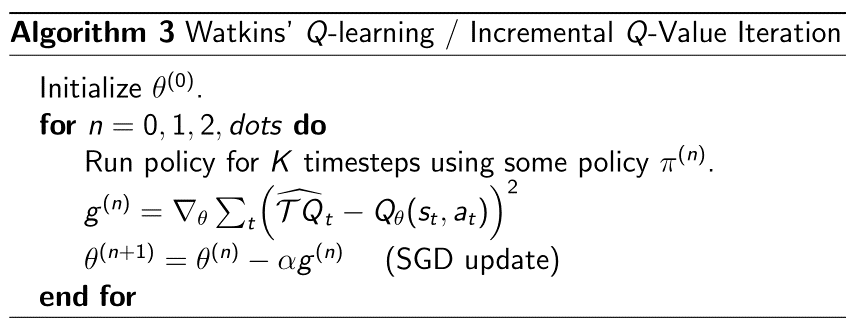
\includegraphics[width=\linewidth]{wat}
  \caption{Incremental Q-Value Iteration}
\end{marginfigure}

\begin{fullwidth}
Q-Value Iteration requires some boundary conditions such as the reward received at the final state of the episode being $0$. In Go or Chess, a $+1$ reward is usually assigned to the transitions that lead to a final winning board (respectively $-1$ for a loosing board) and $0$ for everything else. Hence, the states close to the terminal states are the first to converge because they are close to the \emph{true} label, victory or defeat. The algorithm will diffuse the Q-values for the more distant states between the two extremes $[-1;1]$, and a transition with Q value near to 0 will lead to a balanced board, while the closer to $1$ the closer to a certain victory. As long as we see enough transitions near the terminal states, Q-learning will work reasonably well. Using a function approximator means it will be able to generalize its learning from visited states to states never seen while training. The network should be able to abstract patterns and understand the strength of an action based on previously seen patterns.
\end{fullwidth}

%==============================================================================
\section{DQN}
%==============================================================================
The algorithm, shown below (as copied from the paper) is a hybrid of online  and batch Q-value iteration, interleaving optimization with data collection.
\vspace{-5pt}
\begin{figure}[h]
  \centering
  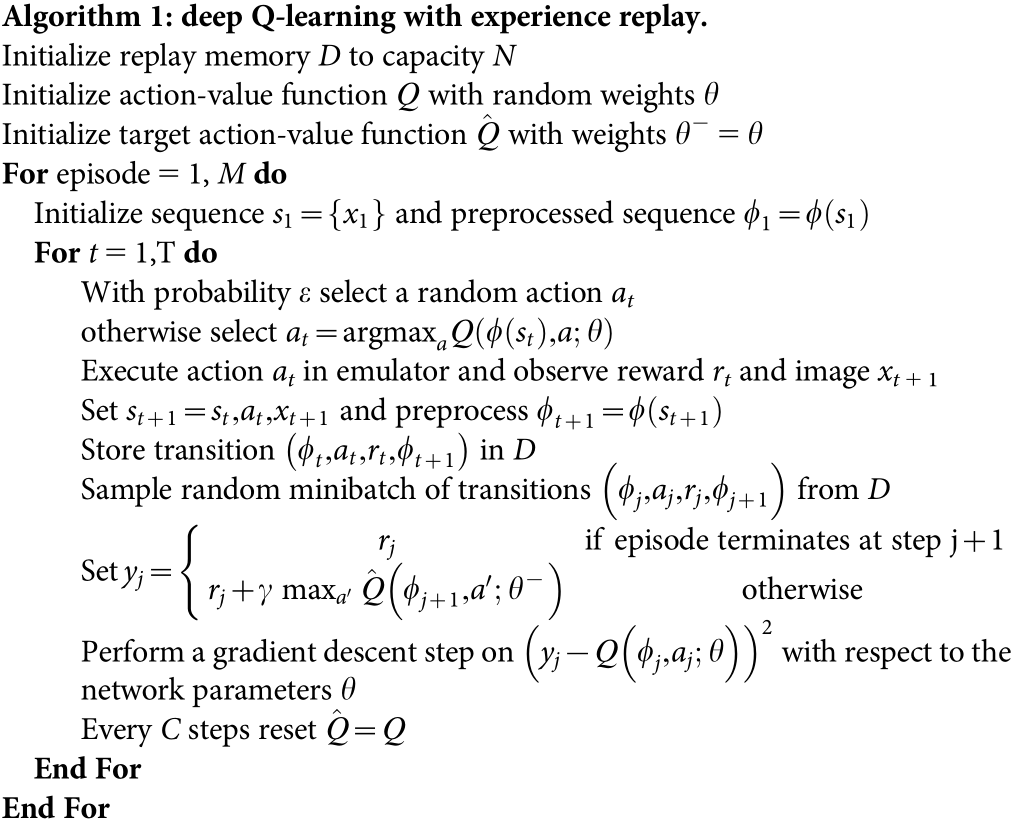
\includegraphics[width=\linewidth]{dqn}
  \label{fig:dqn}
\end{figure}

\marginnote[-7.5cm]{ $\phi_t$ is the processed state, we can just think of it as $s_t$ to maintain consistency with our notation so far.}

\vspace{-5pt}
The major improvements introduced or additions to the vanilla Q-value iteration are described in the following subsections, roughly in order of importance. 

%----------------------------------------------------------
\subsection{Experience Replay}
%----------------------------------------------------------
One of the issues with the vanilla Q-Value iteration algorithm is that the transitions are very correlated. After all, they are extracted from the same episode! The experience replay is a buffer of the last N transition (a million in original paper), from which you randomly sample a minibatch (say 32 transitions) and use this to compute the update (instead of the last transition only). 
\marginnote[-2cm]{Why is this a valid approach? Because, as seen before, the backup $\mathcal{T} Q^{(n)}$ can be performed using off-policy data - so these can be transitions generated by past iterations of the policy we're optimizing.}

Moreover, now the algorithm sees each transition $(s,a,r,s')$ more than once, leading to better data efficiency and reward propagation~\sidenote{Remember, the reward has to be propagated from the states where you actually receive it, backwards. You actually score in Pong many frames after the one in which you actually hit the ball correctly!}. Also, there is increased stability as this history contains data from many past policies derived from  $Q^{(n)},Q^{(n-1)},Q^{(n-2)}, \ldots$ and because it changes rather slowly. 

%----------------------------------------------------------
\subsection{Target network}
%----------------------------------------------------------
The second major addition is the use of a second network during the training procedure:
\begin{itemize}
  \item[$\mathbf{Q}$] is used to select actions and to compute the gradient descent step on at every time step
  \item[$\mathbf{\hat{}Q}$] is the \emph{target} network, a second $Q$ used to compute the Bellman backups, the target Q-values you are trying to get closer to (the further away, the bigger the loss in SGD).
\end{itemize}

Why not just use the current $Q$ as backup target? The issue is that at every training step, the Q-network's values shift, and if we are using a constantly shifting set of values to adjust our network values, then the value estimations can easily spiral out of control. \marginnote{Instead of updating the target network periodically and all at once, it is better to update it frequently, but slowly. This technique was introduced in another DeepMind paper, where they found that it stabilized the training process. \cite{Lillicrap2015-lh}}The network can become destabilized by falling into feedback loops between the target and estimated Q-values. To mitigate that risk, the target network's weights are fixed, and only periodically (every C steps) updated to the primary Q-networks values. Chasing a fixed target is easier than a moving one, and thus training will be more stable. 

%----------------------------------------------------------
\subsection{Exploration vs. exploitation}
%----------------------------------------------------------
Exploring randomly will eventually converge to the optimal policy ... but only after almost infinite time. Usually the state space is too big to visit every possible trajectory, and thus we should try to focus the exploration on the more relevant parts of the state space. A common way (also used here) is $\epsilon-$greedy exploration: choose an action at random with a small probability $\epsilon$ or the best action according to the current policy otherwise \sidenote{$\epsilon $ is usually annealed over time to transition from exploration to exploitation}. 

%----------------------------------------------------------
\subsection{Network architecture}
%----------------------------------------------------------
\begin{figure}[h]
  \centering
  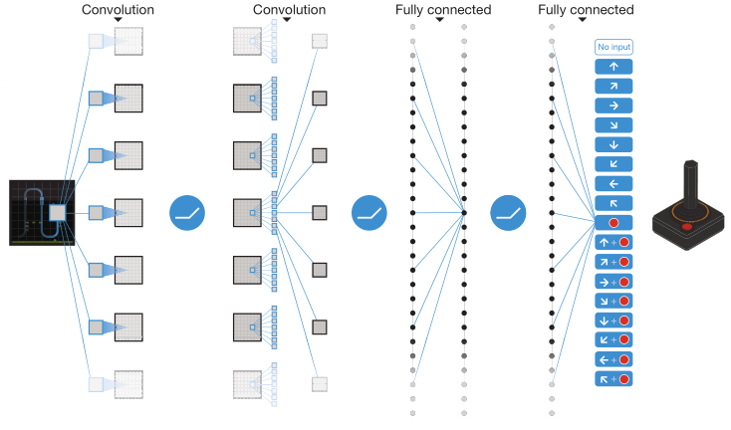
\includegraphics[width=\linewidth]{dqn-net}
  \label{fig:dqn-net}
\end{figure}

The two convolutional layers have 32 8x8 filters with stride 4 and 64 3x3 filters with stride 1. Afterwards there are two fully connected layers of 512 and 18 units, respectively. Each hidden layer is followed by a rectifier nonlinearity. 

The input images are resized to $84\times84$ grayscale, and only 1 in 4 frames is actually processed. For the following 3 images, the last action is repeated. To give information to the network about the current momentum, the last 4 frames (with skip frame, you pick 1 every 4) are stacked into 4 channels. Those 4 frames represent a history we need to construct\sidenote[][-1cm]{A screen snapshot is a partial observation of the full state, since we do not have access to speed vectors for example. Partially observed MDPs (POMDPs) can be reduced to fully observed MDPs by accumulating all previous states into a history. We make do with the last few observations.}, as we are not using Recurrent Neural Networks (RNNs). So we need 16 game frames to construct our $84\times84\times4$ input. The output contains the Q value of every action possible (in different games some of these will be disabled, the minimum and maximum number of actions are 4 and 18). 

%----------------------------------------------------------
\subsection{Results}
%----------------------------------------------------------
\vspace{-10pt}
\begin{figure}[h]
  \centering
  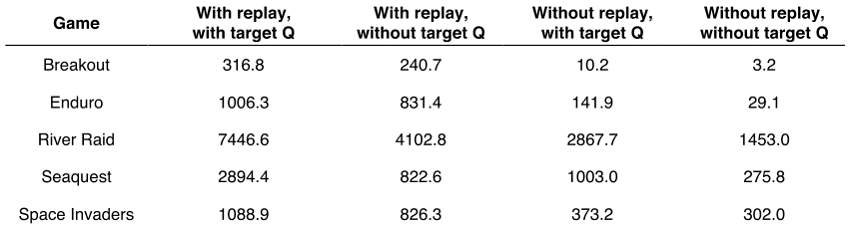
\includegraphics[width=0.9\linewidth]{res1}
\end{figure}


\begin{marginfigure}[-2.5cm]
  \centering
  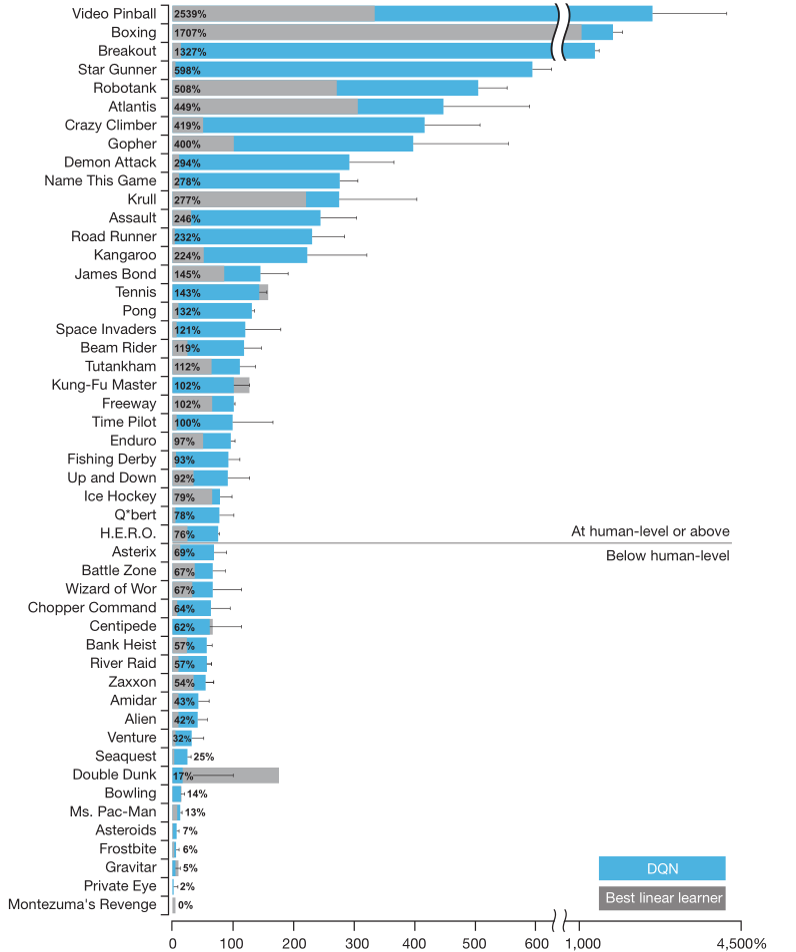
\includegraphics[width=1.2\linewidth]{res2}
\end{marginfigure}

TODO: more text explaining results. Better ($\ge 75\%$) than humans in more than half of the games. Result on the right are scaled from $0\%$-- random play to $100\%$-- professional human games tester.

%----------------------------------------------------------
\subsection{Are Q-Values meaningful?}
%----------------------------------------------------------
\begin{figure}[h]
  \centering
  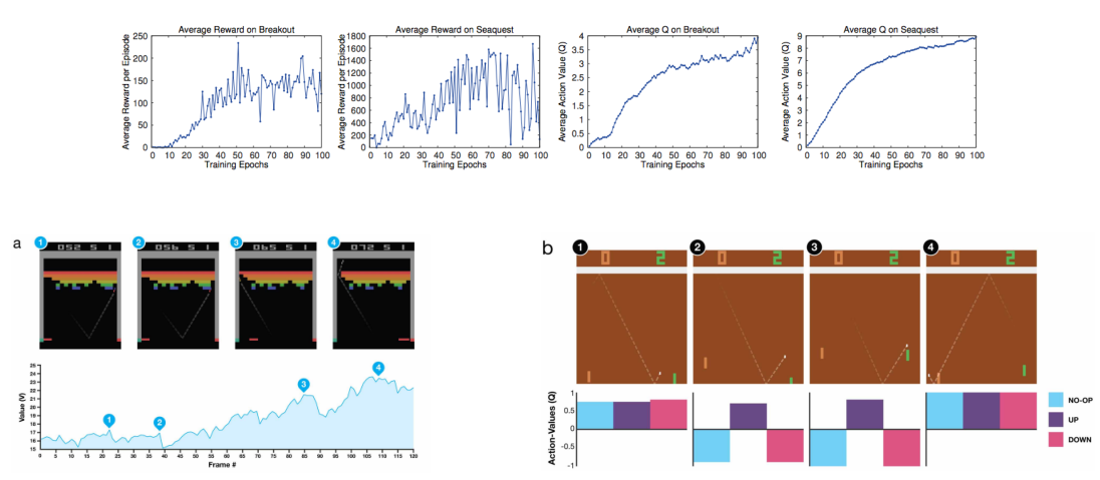
\includegraphics[width=\linewidth]{qval}
\end{figure}

\marginnote[-4cm]{Yes, but usually Q ends up severely overestimating the actual returns. Also, it can shift a lot without significant impact to the loss. Double DQN addresses this. However, DQN works decently in practice because the differences between the Q-value of different actions is more important than their absolute value. \cite{Van_Hasselt2015-ry}}

%==============================================================================
\section{Conclusions}
%==============================================================================
\begin{itemize}
  \item Single architecture (same algorithm, network architecture and hyperparameters) used to learn control policies for 49 different environments.
  \item Minimal prior knowledge, only pixels and score as input.
  \item Not equally reliable on all tasks.
    \begin{figure}[h]
      \centering
      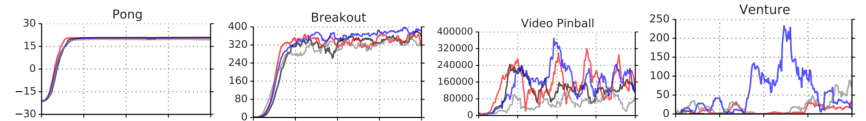
\includegraphics[width=\linewidth]{reliable}
    \end{figure}
  \item Improvements from recent work (to be discussed later)
    \begin{itemize}
      \item Double DQN: closer DQN estimates to true values
      \item Dueling nets: separately estimate V and A, $Q(s,a)=V(s) + A(s,a)$) 
      \item Prioritized replay: favor important time steps - large gradients
    \end{itemize}
\end{itemize}

Some other tips:
\begin{itemize}
\item Large replay buffers (~1 M) improve robustness.
\item Converges slowly: ATARI often needs 10-40M frames (hours on a GPU) to get better than a random policy.
\item Run at least 2-3 different seeds when experimenting.
\item Learning rate scheduling is important (high rates in initial exploration, decrease over time).
\end{itemize}

\bibliography{references}
\bibliographystyle{plainnat}
% \bibliographystyle{ieeetr}

\end{document}
